\documentclass{standalone}
\usepackage{fontspec}
\setsansfont{DejaVuSans.ttf}[Path=./,Kerning=Off,Ligatures={TeXOff,NoCommon}]
\usepackage{tikz}
\begin{document}
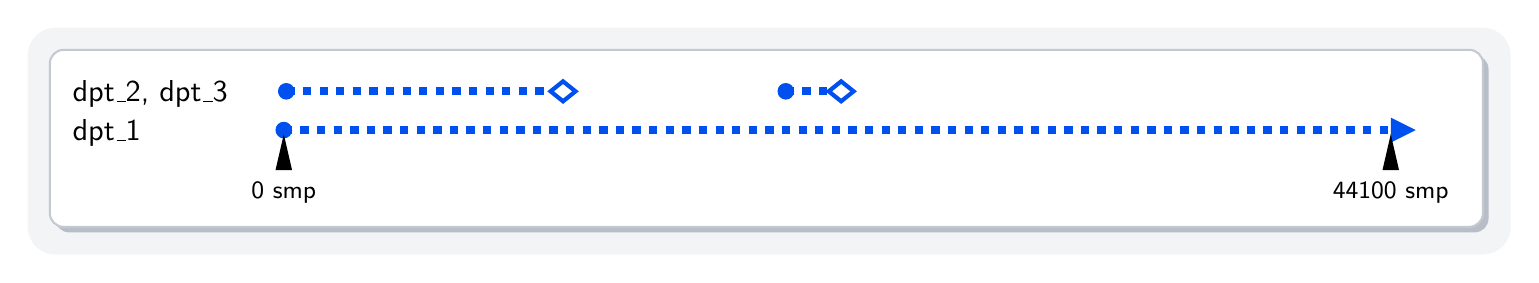
\begin{tikzpicture}[x=1pt,y=1pt,miter limit=4,font=\sffamily]
\definecolor{ts000000}{HTML}{000000}
\definecolor{ts0050EF}{HTML}{0050EF}
\definecolor{tsB8BEC8}{HTML}{B8BEC8}
\definecolor{tsC4C9D1}{HTML}{C4C9D1}
\definecolor{tsF3F4F6}{HTML}{F3F4F6}
\definecolor{tsFFFFFF}{HTML}{FFFFFF}
\begin{scope}[shift={(16,16)}]
\path[rounded corners=10pt,fill=tsF3F4F6] (0,0) rectangle (535.876,81.9766);
\path[rounded corners=5pt,fill=tsB8BEC8] (10,8) rectangle (527.876,71.9766);
\path[rounded corners=5pt,fill=tsFFFFFF,draw=tsC4C9D1,line width=0.75pt] (8,10) rectangle (525.876,73.9766);
\path[draw=ts0050EF,line width=3pt,dash pattern=on 3pt off 3pt] (92.5459,44.9766) -- (492.5459,44.9766);
\path[fill=ts0050EF] (92.5459,44.9766) circle[radius=3];
\path[fill=ts0050EF] (501.5459,44.9766) -- (492.5459,49.4766) -- (492.5459,40.4766) -- cycle;
\path[draw=ts0050EF,line width=3pt,dash pattern=on 3pt off 3pt] (93.4529,58.9766) -- (188.9529,58.9766);
\path[fill=ts0050EF] (93.4529,58.9766) circle[radius=3];
\path[draw=ts0050EF,line width=1.5pt] (188.9529,58.9766) -- (193.4529,62.5766) -- (197.9529,58.9766) -- (193.4529,55.3766) -- cycle;
\path[draw=ts0050EF,line width=3pt,dash pattern=on 3pt off 3pt] (273.9518,58.9766) -- (289.4518,58.9766);
\path[fill=ts0050EF] (273.9518,58.9766) circle[radius=3];
\path[draw=ts0050EF,line width=1.5pt] (289.4518,58.9766) -- (293.9518,62.5766) -- (298.4518,58.9766) -- (293.9518,55.3766) -- cycle;
\path[fill=ts000000] (92.5459,43.4766) -- (89.5459,30.4766) -- (95.5459,30.4766) -- cycle;
\path[fill=ts000000] (492.5459,43.4766) -- (489.5459,30.4766) -- (495.5459,30.4766) -- cycle;
\node[anchor=base west,inner sep=0,font=\sffamily\fontsize{11}{12.8047}\selectfont,text=ts000000] at (16,55.1685) {dpt\_2, dpt\_3};
\node[anchor=base west,inner sep=0,font=\sffamily\fontsize{11}{12.8047}\selectfont,text=ts000000] at (16,41.1685) {dpt\_1};
\node[anchor=base,inner sep=0,font=\sffamily\fontsize{9}{10.4766}\selectfont,text=ts000000] at (92.5459,20.1226) {0 smp};
\node[anchor=base,inner sep=0,font=\sffamily\fontsize{9}{10.4766}\selectfont,text=ts000000] at (492.5459,20.1226) {44100 smp};
\end{scope}
\end{tikzpicture}
\end{document}
